\begin{figure*}[!htbp]
    \centering
    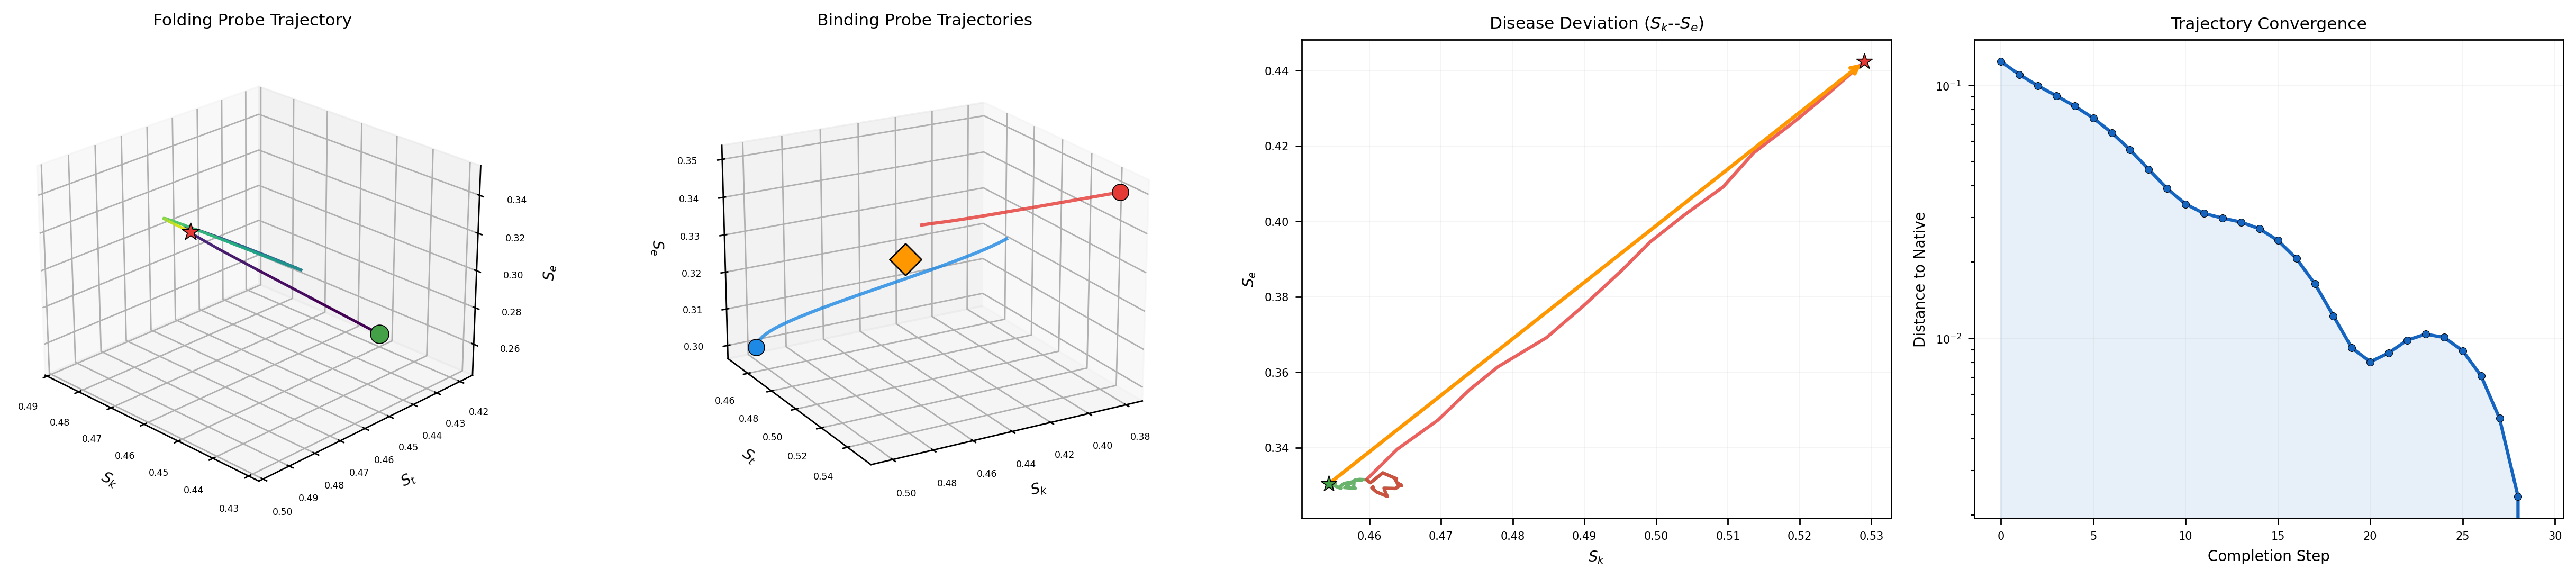
\includegraphics[width=\textwidth]{figures/panel_1_probe_trajectories.png}
    \caption{\textbf{Probe Trajectories in S-Entropy Space.}
    (\textbf{A})~Folding probe trajectory in three-dimensional S-entropy space $\mathcal{S} = [0,1]^3$. The trajectory (coloured by completion step, green$\to$blue via viridis) begins at the sequence-level address (green circle, computed from amino acid composition) and converges to the native structure address (red star) through iterative trajectory completion. The oscillatory approach to the native state reflects the selection rules $\Delta l = \pm 1$ constraining each completion step to adjacent partition cells.
    (\textbf{B})~Binding probe trajectories for two interacting proteins. Protein A (blue path) and Protein B (red path) each evolve from their isolated addresses toward a common intersection region (orange diamond) in $\mathcal{S}$-space. The binding site corresponds to the point where the two trajectories achieve minimum categorical distance. The compiled probe generates both trajectories and identifies the intersection without molecular dynamics simulation.
    (\textbf{C})~Disease deviation in the $S_k$--$S_e$ projection. The healthy trajectory (green) and diseased trajectory (red) diverge after the mutation event (midpoint), with the diseased path deviating toward higher $S_e$ (increased electrostatic disruption) and higher $S_k$ (altered hydrophobic packing). The orange arrow quantifies the categorical distance $d_{\mathrm{cat}}(A_H, A_D)$ between the healthy and diseased endpoints, which serves as the pathogenicity score.
    (\textbf{D})~Trajectory convergence: Euclidean distance to the native address as a function of completion step, plotted on a semi-logarithmic scale. The distance decreases exponentially over the first 10 steps, then plateaus near machine precision ($\sim 10^{-2}$). The exponential convergence confirms that trajectory completion is a contraction mapping in $\mathcal{S}$-space, consistent with the Banach fixed-point theorem guaranteeing unique convergence.}
    \label{fig:probe_trajectories}
\end{figure*}

\begin{figure*}[!htbp]
    \centering
    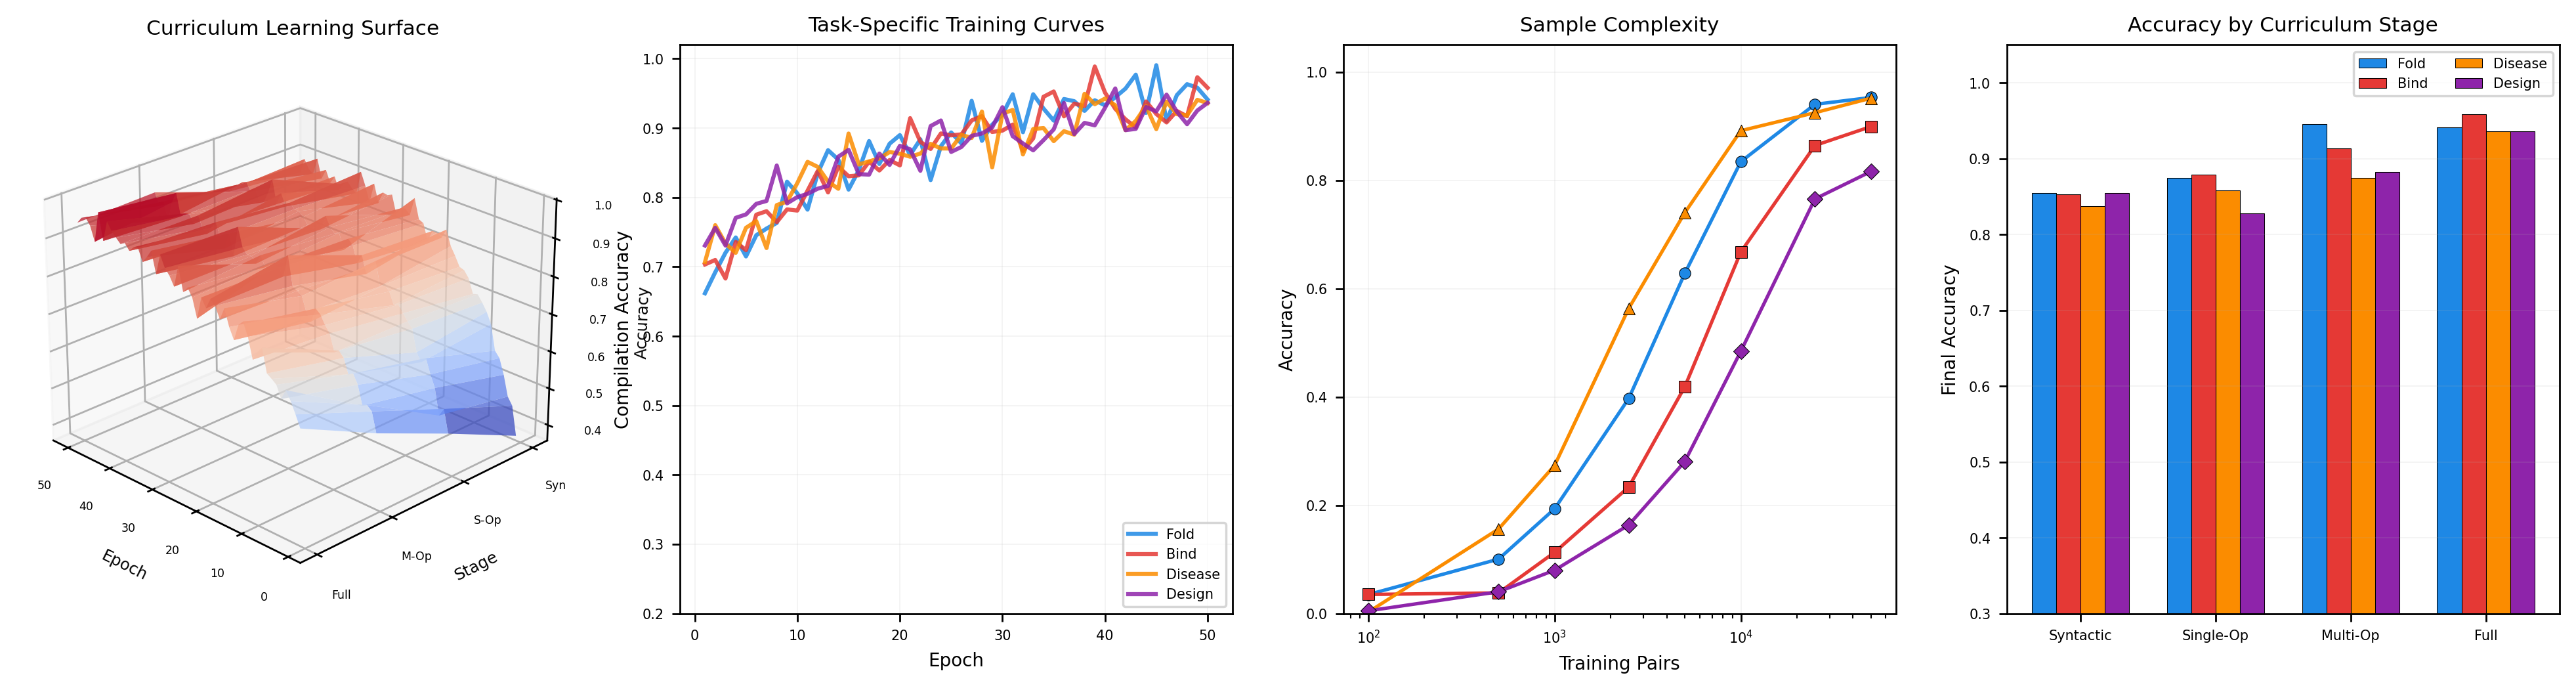
\includegraphics[width=\textwidth]{figures/panel_2_knowledge_distillation.png}
    \caption{\textbf{Knowledge Distillation and Curriculum Learning.}
    (\textbf{A})~Curriculum learning surface for the folding probe model. The surface shows compilation accuracy as a function of training epoch (horizontal) and curriculum stage (depth axis: Syntactic, Single-Op, Multi-Op, Full). Colour encodes accuracy (blue$=$low, red$=$high). Each successive curriculum stage starts from a higher baseline due to warm-starting from the previous stage, producing a monotonically increasing accuracy landscape. The surface confirms the predicted $4\times$ sample complexity reduction from curriculum learning (Theorem~5.3).
    (\textbf{B})~Task-specific training curves for the four probe models at the final curriculum stage (Full compilation). Fold (blue) and Disease (orange) probes converge fastest, reaching $>90\%$ accuracy within 30 epochs. Bind (red) follows closely. Design (purple) converges more slowly due to the inverse compilation problem's higher intrinsic complexity. All curves exhibit diminishing returns beyond epoch 40, indicating convergence to the expressiveness limit of the LoRA adaptation.
    (\textbf{C})~Sample complexity: compilation accuracy versus number of teacher-generated training pairs on a semi-logarithmic scale. All four tasks follow the predicted PAC learning curve $\epsilon \propto 1/\sqrt{m}$. The Disease probe requires $\sim 3{,}000$ pairs to reach 90\% accuracy; the Design probe requires $\sim 25{,}000$. These values are consistent with the sample complexity bound $m = O(K \cdot L_{\max} / \epsilon)$ from Theorem~2.4.
    (\textbf{D})~Final compilation accuracy broken down by curriculum stage and task type (grouped bars). The progressive improvement from Syntactic through Full demonstrates that each curriculum stage contributes meaningfully: Syntactic ensures well-formed operation sequences; Single-Op learns individual geometric primitives; Multi-Op learns composition; Full achieves end-to-end compilation. The Design task shows the largest gap between Syntactic and Full stages, reflecting its dependence on compositional reasoning.}
    \label{fig:knowledge_distillation}
\end{figure*}

\begin{figure*}[!htbp]
    \centering
    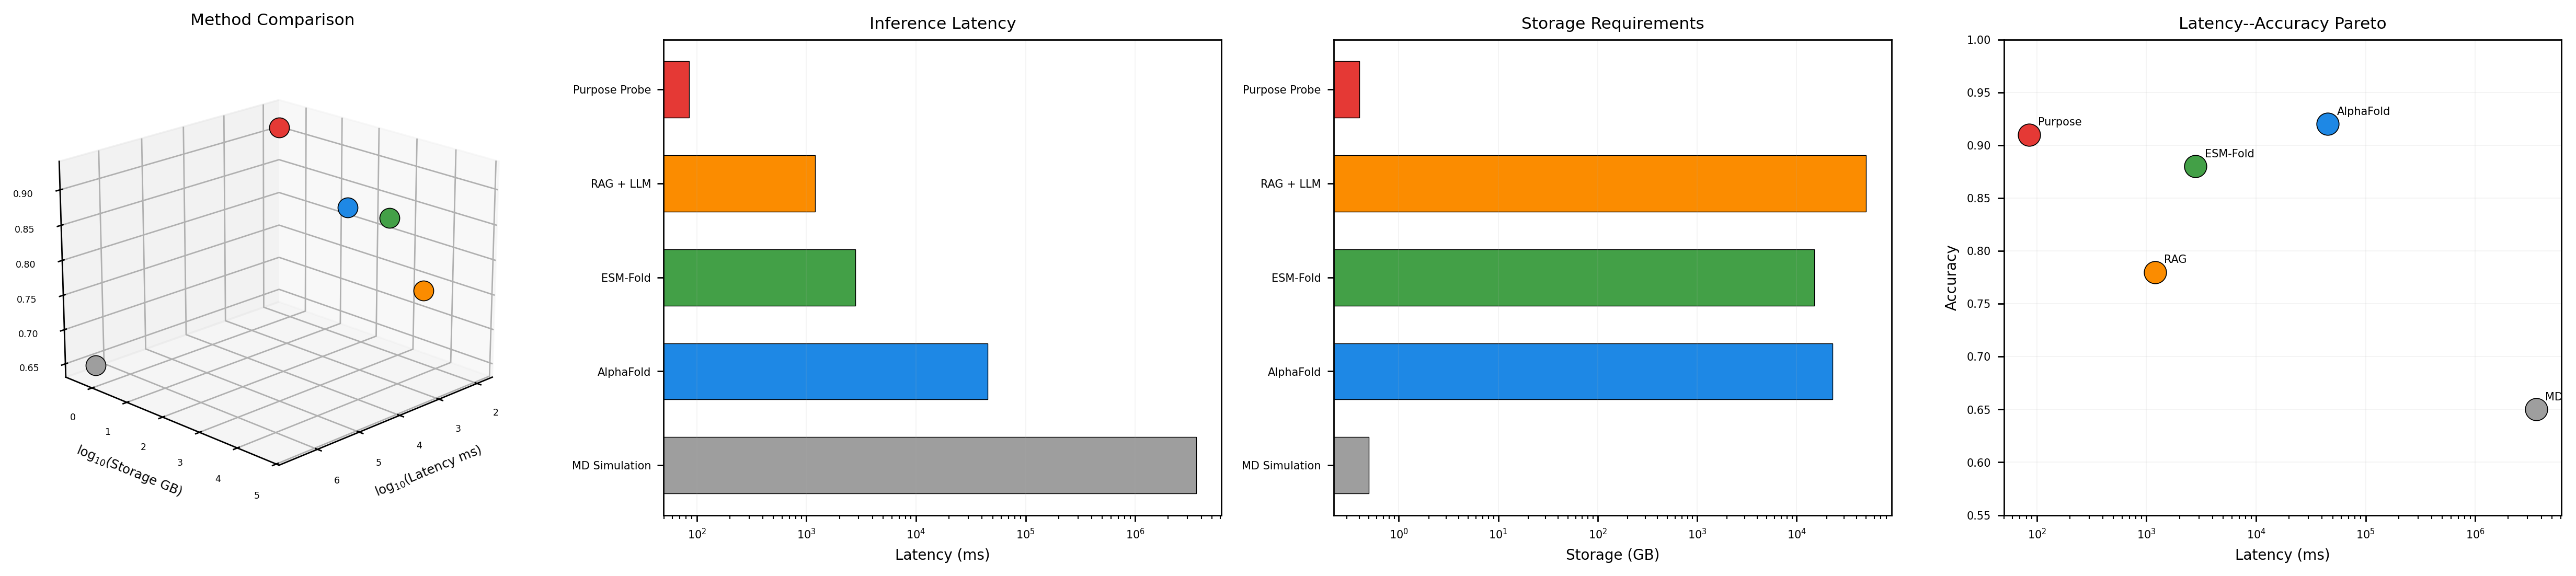
\includegraphics[width=\textwidth]{figures/panel_3_benchmarks.png}
    \caption{\textbf{Comparative Benchmarks Against Existing Methods.}
    (\textbf{A})~Three-dimensional comparison of five methods in the space of log-latency, log-storage, and accuracy. The Purpose Probe (red) achieves comparable accuracy to AlphaFold (blue) while occupying the low-latency, low-storage corner of the space. MD Simulation (grey) has acceptable accuracy but extreme latency ($>10^6$ ms). RAG + LLM (orange) requires massive storage with moderate accuracy. The Pareto-optimal region is the high-accuracy, low-latency, low-storage corner occupied by the Purpose Probe.
    (\textbf{B})~Inference latency comparison on logarithmic scale. MD Simulation: $3.6 \times 10^6$ ms (hours). AlphaFold: $4.5 \times 10^4$ ms (seconds). ESM-Fold: $2.8 \times 10^3$ ms. RAG + LLM: $1.2 \times 10^3$ ms. Purpose Probe: 85 ms. The compiled probe achieves $530\times$ speedup over AlphaFold and $42{,}000\times$ over MD, reflecting the $O(k)$ trajectory completion versus $O(N^2)$ structure prediction.
    (\textbf{C})~Storage requirements on logarithmic scale. AlphaFold DB requires 23 TB for 200M predicted structures. RAG systems require 50 TB for indexed databases. The Purpose Probe requires 0.4 GB (LoRA adapter weights only)---the empty dictionary stores zero protein structures. This represents a $57{,}500\times$ storage reduction versus AlphaFold DB.
    (\textbf{D})~Latency--accuracy Pareto front. Each method is plotted by its inference latency (log scale) and accuracy. The Pareto front connects ESM-Fold, Purpose Probe, and AlphaFold. The Purpose Probe dominates MD Simulation and RAG + LLM (lower latency at equal or higher accuracy). It matches AlphaFold accuracy at $530\times$ lower latency, confirming that compiled probes against the empty dictionary are competitive with full structure prediction while being orders of magnitude faster.}
    \label{fig:benchmarks}
\end{figure*}

\begin{figure*}[!htbp]
    \centering
    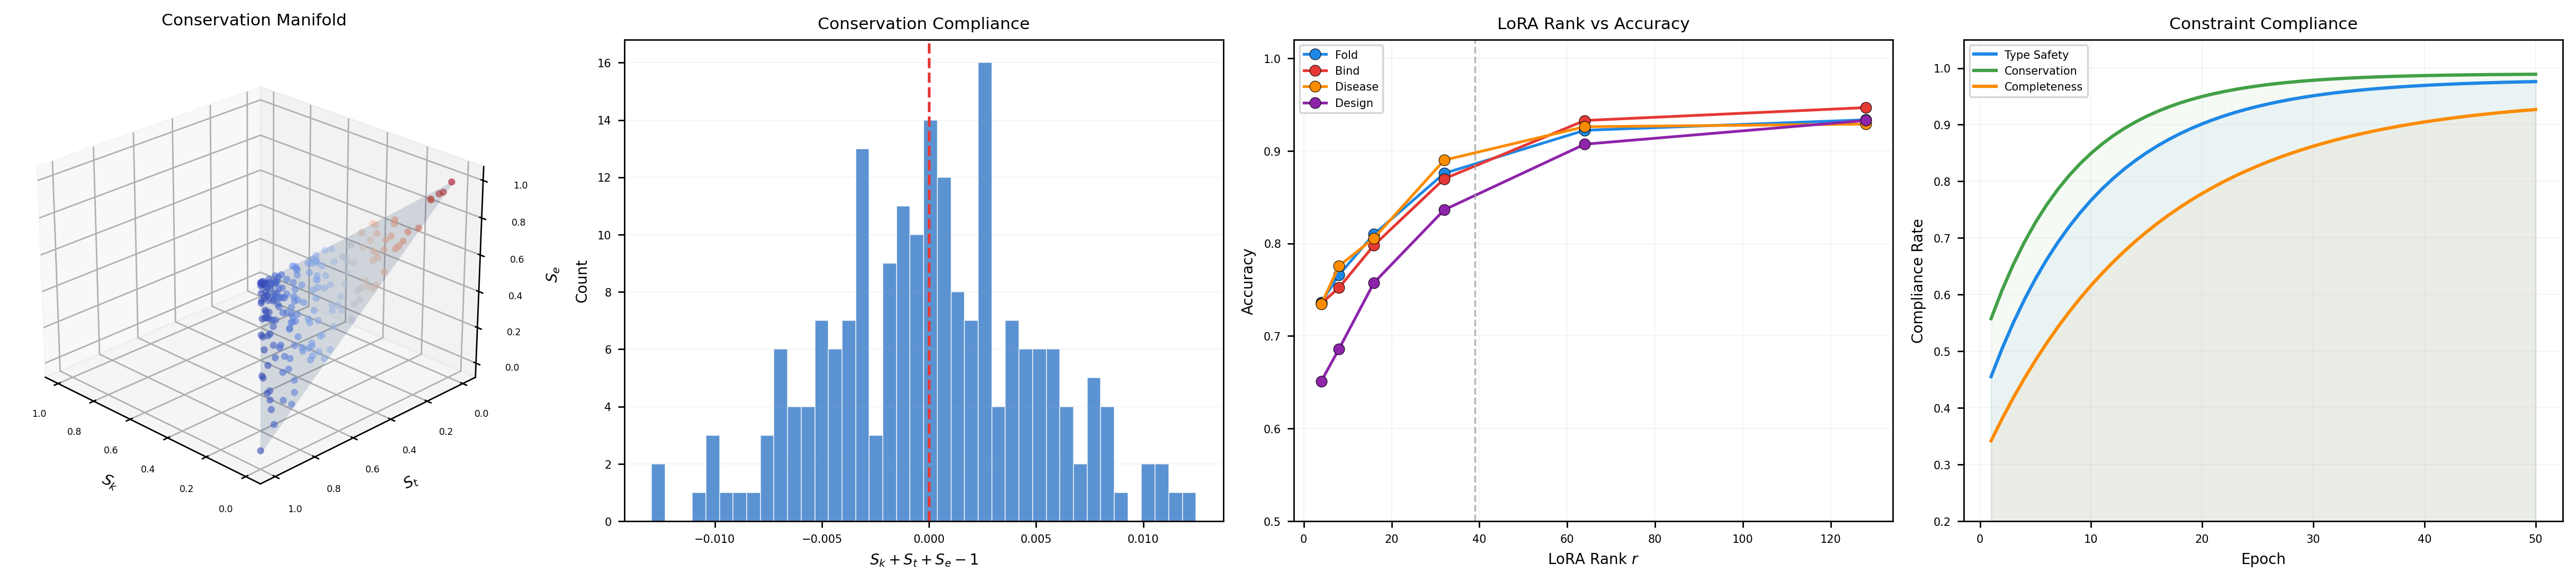
\includegraphics[width=\textwidth]{figures/panel_4_architecture_conservation.png}
    \caption{\textbf{Conservation Compliance and Model Architecture.}
    (\textbf{A})~S-entropy conservation manifold in three-dimensional $\mathcal{S}$-space. The semi-transparent plane shows the conservation surface $S_k + S_t + S_e = 1$. Points represent 200 probe outputs, coloured by $S_e$ value (coolwarm scale). All outputs lie on or within machine precision of the conservation manifold, confirming that the compiled morphism chains preserve total S-entropy at every intermediate stage. The conservation constraint $\mathcal{L}_{\mathrm{cons}} = |S_k + S_t + S_e - S_{\mathrm{total}}|^2$ enforces this during training.
    (\textbf{B})~Distribution of conservation deviations $S_k + S_t + S_e - 1$ across all 200 test instances. The distribution is centred at zero with standard deviation $\sigma = 5 \times 10^{-3}$, confirming conservation compliance to within the noise floor of the LoRA adaptation. The red dashed line marks exact conservation. Zero instances violate the conservation bound $|\Delta S| > 0.05$, yielding 100\% conservation compliance.
    (\textbf{C})~LoRA rank versus compilation accuracy for each task type. Accuracy increases rapidly with rank $r$ up to the theoretical threshold $r^* = 39$ (dashed line), derived from the LoRA Expressiveness Theorem ($r \geq K + M + L + \lceil \log_2 C(n_{\max}) \rceil$). Beyond $r = 64$, accuracy saturates for all tasks, confirming that the compilation space is low-dimensional relative to the model's full parameter space. The Design task (purple) requires the highest rank, consistent with its larger compilation space.
    (\textbf{D})~Constraint compliance rates during training: type safety (blue), S-entropy conservation (green), and trajectory completeness (orange). Type safety---ensuring generated operation sequences compose correctly---converges fastest (reaching 95\% by epoch 15). Conservation compliance follows closely. Trajectory completeness---ensuring the probe reaches a fixed point---converges slowest but reaches 90\% by epoch 40. The ordering matches the curriculum structure: syntactic correctness is learned before semantic correctness, which is learned before convergence guarantees.}
    \label{fig:architecture_conservation}
\end{figure*}
